\documentclass{article}
\usepackage[utf8]{inputenc}
\usepackage[T1]{fontenc}
\usepackage{graphicx}
\usepackage{color}
\usepackage{amsmath}
\usepackage{caption}
\usepackage{wrapfig}
\usepackage{tikz}
\usepackage[none]{hyphenat}

\title{Pythagorean Theorem}
\author{1505080}
\date{\today}

\usepackage{natbib}
\usepackage{graphicx}

\begin{document}

\maketitle

\section{Introduction}
    In this document, we present the very famous theorem in mathematics: Pythagorean theorem, which is stated as follows.\\
    \\
    \textbf{Theorem 1.1 (Pythagorean theorem) } \textit{The square of the hypotenuse (the side opposite the right angle) is equal to the sum of the squares of the other two sides.} \\
    \par
    Numerous mathematicians proposed various proofs to the theorem. The theorem was long known even before the time of Pythagoras. Pythagoras was the first to provide with a sound proof. The proof that Pythagoras gave was by \textit{rearrangement}. Even the great Albert Einstein also proved the theorem without rearrangement, rather by using dissection. Figure \ref{fig:pythThmFig1} shows the visual representation of the theorem.

    \begin{figure}[h!]
        \centering
        
        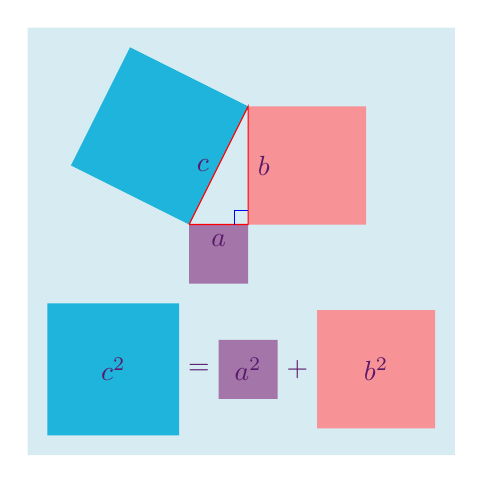
\begin{tikzpicture}[scale = 0.5]
            % \draw [help lines,step = 1 cm] (-10,-10) grid (10,10);
            % \draw (-10,0) -- (10,0);   
            % \draw (0,-10) -- (0,10);
            
            \definecolor{fillColor}{RGB}{215,235,242};
            \path [fill = fillColor] (-4.099101966,-5.854101966) -- (-4.099101966,5) -- (6.75,5) -- (6.75,-5.854101966) -- (-4.099101966,-5.854101966);
            
            
            \definecolor{aColor}{RGB}{164,117,169};
            \path [fill = aColor] (0,0) -- (1.5,0) -- (1.5,-1.5) -- (0,-1.5) -- (0,0);
            
            \definecolor{bColor}{RGB}{247,146,150};
            \path [fill = bColor] (1.5,0) -- (1.5,3) -- (4.5,3) -- (4.5,0) -- (1.5,0);
            
            \definecolor{cColor}{RGB}{30,180,220};
            \path [fill = cColor] (0,0) -- (-3,1.5) -- (-1.5,4.5) -- (1.5,3) -- (0,0);
            
            \draw[red] (0,0) -- (1.5,0) -- (1.5,3) -- (0,0);
            \draw[blue] (1.5,0.35) -- (1.15,0.35) -- (1.15,0);
            
            \definecolor{nodeColor}{RGB}{90,26,107};
            
            \node [below, nodeColor] at (0.75,0) {$a$};
            \node [right, nodeColor] at (1.5,1.5) {$b$};
            \node [left, nodeColor] at (0.75,1.5) {$c$};
            
            
            
            \path [fill = aColor] (0.75,-2.927050983) -- (2.25,-2.927050983) -- (2.25,-4.427050983) -- (0.75,-4.427050983) -- (0.75,-2.927050983);  
            \node [nodeColor] at (1.5,-3.677050983) {$a^2$};
            
            \node [nodeColor] at (2.75,-3.677050983) {$+$};
            
            \path [fill = bColor] (3.25,-2.177050983) -- (6.25,-2.177050983) -- (6.25,-5.177050983) -- (3.25,-5.177050983) -- (3.25,-2.177050983);  
            \node [nodeColor] at (4.75,-3.677050983) {$b^2$};
            
            \node [nodeColor] at (0.25,-3.677050983) {$=$};
            
            \path [fill = cColor] (-3.599101966,-2) -- (-.25,-2) -- (-.25,-5.354101966) -- (-3.599101966,-5.354101966) -- (-3.599101966,-2);  
            \node [nodeColor] at (-1.922050983,-3.677050983) {$c^2$};
            
            
        
        \end{tikzpicture}
        
        \caption{Visual representation of the famous Pythagorean theorem.}
        \label{fig:pythThmFig1}
    \end{figure}



    \begin{figure}[h!]
        \centering
        
        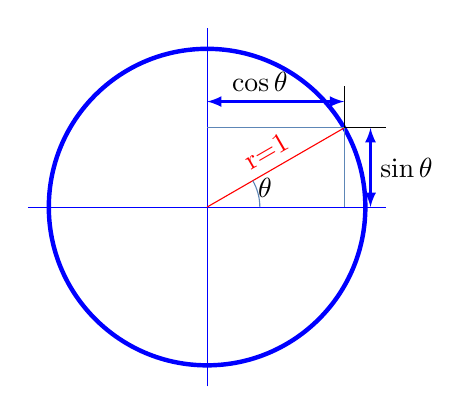
\begin{tikzpicture}[scale = 0.67]
            %\draw [step = 1 cm, help lines] (-5,-5) grid (5,5);
            \draw [blue, ultra thin] (-3.398076211,0) -- (3.398076211,0);   
            \draw [blue, ultra thin] (0,-3.398076211) -- (0,3.398076211);
            
            \draw [blue, ultra thick] (0,0) circle (3);
            
            \draw [red] (0,0) -- (2.598076211, 1.5);
            \definecolor{arcColor}{RGB}{93,134,182}

            \draw [arcColor] (1,0) arc [radius = 1, start angle =0, end angle = 30];
            
            \draw [arcColor] (0,1.5) -- (2.598076211, 1.5) -- ( 2.598076211,0); 
            
            \draw[black] (2.598076211, 1.5) -- (3.398076211, 1.5);
            \draw[black] (2.598076211, 1.5) -- (2.598076211, 2.3);
            
            \draw[blue, thick, <->, >=latex] (0,2) -- (2.598076211, 2);
            \draw[blue, thick, <->, >=latex] ( 3.098076211,0) -- (3.098076211, 1.5);
            
            \node [above] at (1,2) {$\cos{\theta}$};
            \node [right] at (3.098076211,0.75) {$\sin{\theta}$};
            \node [above] at (1.1,0) {$\theta$};
            
            \node[rotate = 30, red, above] at (1.299038106, 0.75) {r=1};
            
            
        \end{tikzpicture}
        
        \caption{Alternate representation of Pythagorean theorem.}
        \label{fig:pythThmFig2}
    \end{figure}

\section{Trigonometric Forms}
    Lots of other forms of the same theorem exist. The most useful, perhaps, are expressed in trigonometric terms, as follows: 

    \begin{equation}
            \sin^2\theta + \cos^2\theta = 1
            \label{eqn:pythThmEqn1}
    \end{equation}
    
    \begin{equation}
            \sec^2\theta - \tan^2\theta = 1
            \label{eqn:pythThmEqn2}
    \end{equation}
    
    \begin{equation}
            \mathrm{cosec}^2\theta - \cot^2\theta = 1
            \label{eqn:pythThmEqn3}
    \end{equation}

    \subsection{Representing the First}
        Taking \ref{eqn:pythThmEqn1}, we can show them as shown in Figure\ref{fig:pythThmFig2}. When we take a point at unit distance from the origin, the $y$ and $x$ co-ordinates become $\sin\theta$ and $\cos\theta$ respectively. Therefore, sum of the squares of the two becomes equal to the square of the unit distance, which, of course, is 1.
    

\end{document}



